\documentclass[11pt]{article}
\pdfinfoomitdate=1\pdftrailerid{}
\usepackage[letterpaper,margin=.7in,headheight=15pt,headsep=18pt,footskip=24pt]{geometry}
\usepackage[T1]{fontenc}
\usepackage{lmodern,amsmath,amssymb,array,booktabs,fancyhdr,tikz}
\renewcommand{\familydefault}{\sfdefault}
\setlength{\parindent}{0pt}\setlength{\parskip}{6pt}
\pagestyle{fancy}\fancyhf{}
\fancyhead[L]{\small Week 97 / Square remainders / K--1 adult guide}
\fancyfoot[L]{\scriptsize Bellingham Math Circle / Week 97 / W97-K-FAC-v2}
\fancyfoot[R]{\thepage}
\renewcommand{\headrulewidth}{0pt}
\newcommand{\head}[1]{\par\textbf{\large #1}\par}
\newcommand{\sub}[1]{\par\textbf{#1}\par}
% Generated by check_guide.py from independent enumeration.
\newcommand{\Pone}{1, 0, 1, 0, 1, 0}
\newcommand{\Ptwo}{0:\{2, 4\};\quad 1:\{1, 3, 5\}}
\newcommand{\Pthree}{0, 2, 2, 3}
\newcommand{\Recttotals}{12, 6, 10, 15}
\newcommand{\Pfour}{1, 1, 0, 1, 1, 0}
\newcommand{\Pfive}{1, 4, 3, 4, 1, 0}
\newcommand{\Psix}{0:\{6\};\quad 1:\{1, 5\};\quad 3:\{3\};\quad 4:\{2, 4\}}
\newcommand{\Pseven}{1, 0, 1, 0, 1}
\newcommand{\Peighta}{1}
\newcommand{\Peightb}{0}
\newcommand{\Ringcounts}{8, 16}
\newcommand{\Pten}{1}
\newcommand{\Peleven}{0:\{4\};\quad 1:\{1, 3, 5\};\quad 4:\{2, 6\}}

\begin{document}
\head{Mathematical overview: what a leftover can tell us}
\textbf{Squares restrict the leftovers.} For a filled $n\times n$ square, remove any $m$ tiles at a time until fewer than $m$ remain. Here $n$ is a whole-number side length and $m>0$; the leftover can be zero. The choice of tiles does not affect it. Squares leave only 0 or 1 in groups of 3 or 4, and only 0, 1, 3 or 4 in groups of 6. These restrictions are about squares, not arbitrary piles or rectangles.

\textbf{Why a finite list suffices.} Adding $m$ to a side adds two $n\times m$ strips and an $m\times m$ corner. Each added region splits into whole groups of $m$, so sides $n$ and $n+m$ have the same leftover. Sides 1 through $m$ therefore cover every possibility, including side zero's leftover. The student cards themselves start at 1, not zero. For groups of 4, an even-sided square splits into $2\times2$ blocks. An odd-sided square has an even square inside, two equal even-length arms that pair into groups of 4, and one corner tile: only that corner remains.

\textbf{One result can hide several squares.} For $0\le n\le m$, sides $n$ and $m-n$ have the same leftover in groups of $m$: their square totals differ by $m(m-2n)$, whole groups of $m$. For groups of 6, sides 1 and 5 pair, as do 2 and 4; among cards 1--6, sides 3 and 6 stand alone. In objects, remove a $1\times1$ corner from a $5\times5$ square. Cut the remaining L into a $4\times5$ rectangle and a $1\times4$ strip; turn the strip to make a $4\times6$ rectangle, all whole groups of 6. This is the base guide's L argument (p.\ 5) with different sizes. A secret answer names \emph{all} allowed cards with the observed leftover.

\textbf{A composite surprise.} Groups of 8 allow only 0, 1 and 4, although the group size is composite. Every odd square leaves 1: its rings have $8,16,24,\ldots$ tiles, all full groups, around one middle tile. Groups of 2 leave 0 for even sides and 1 for odd sides. The finite lists for groups of 6 and 8 give contrasting examples of the older tables' prime/composite question (base overview, p.\ 1).

\textbf{Discovery and evidence.} K--1 discovers restricted leftovers, paired hidden inputs and the composite-size comparison. A build is an experiment; ``I think this always happens'' is a conjecture. Checking every allowed card proves a finite game answer. An objects argument can explain a pattern for every side; merely testing more squares does not. Children need no modular notation or multiplication facts.

\head{Preparation and access}
\textbf{Status.} Unpiloted and physically unrehearsed. Tile fit, cutting, screen concealment, card handling, adult procedures and timings still need a real rehearsal.

\textbf{Per pair.} Use the week's 64 counters or square tiles (1-inch square tiles if the room has them), a whiteboard and pen, and scrap paper. Add one cup and one upright folder screen. Two colors are useful for rings; 32 of each suffice. Reuse tiles between builds. The six printed picture cards replace the base kit's hand-marked input cards at this table; no extra deck is needed.

\textbf{Print.} Use the K--1 packet W97-K-v1 (\texttt{week-97-k-1.pdf} once approved; current draft: \texttt{k-1.pdf}). Print task pages 1--11 \emph{per child}, and board page 12 and side-card sheet page 13 \emph{per pair}. Cut page 13 into six 58 by 74\,mm cards. First visit: task pages 1--3 per child, plus 12--13 per pair; keep page 7 available. US Letter, single-sided, Actual Size. The $6\times6$ board is 156\,mm across, with 26\,mm cells; try a 25.4\,mm tile first. Small square pictures show which square to build; they are not mats. Keep the board loose; cut only page 13. Allow 5--10 extra minutes for cutting and fit checks; no separate materials PDF is needed.

\newpage
\head{Launch together, then learn the table action}
Join \emph{only the first part} of the base guide's whole-group launch (p.\ 2): handle tiles, see the $3\times3$ square in groups of 4 and the empty square, and make a legal attempt. \textbf{Take K--1 to its table before the paragraph that reads the printed bundles-of-4 collection.} That paragraph reveals Problem 1's pattern and begins Problem 2's work. At the table: ``input'' is the side, ``bundle'' is a group, ``output'' is the leftover. Page 1's grey 1 records the shared example; it is not a new puzzle.

\textbf{A non-task demonstration, about 3 minutes.} Draw five tile-sized spaces on the whiteboard. This temporary group-of-5 mat is not a student task. Fill a side-4 square on the loose board. Move five tiles onto the mat, then into the cup; do this three times in all. Trying again leaves four spaces empty. The one tile outside the cup is the leftover, whether on the board or the partly filled mat. Record 1 beneath side 4.

\begin{center}
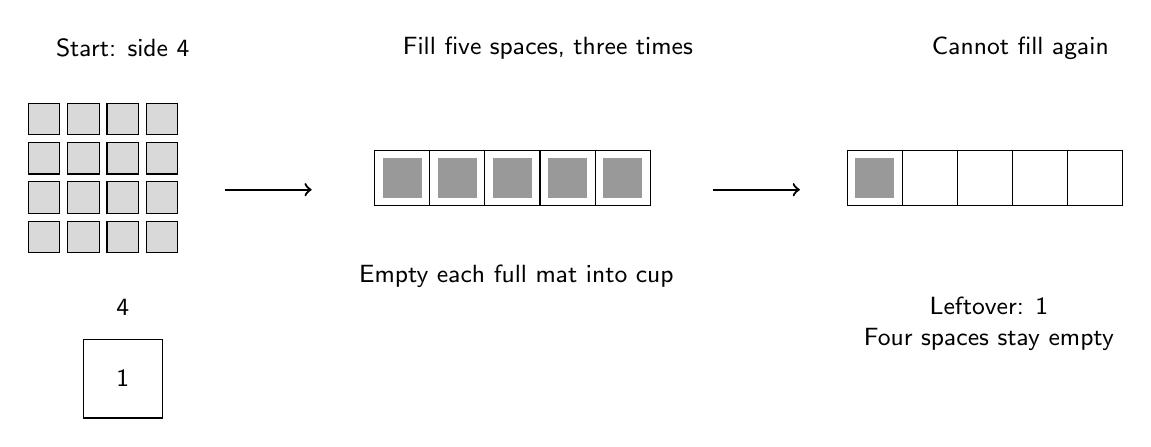
\begin{tikzpicture}[x=1mm,y=1mm,font=\small]
\node at (12,26) {Start: side 4};
\foreach \x in {0,1,2,3}\foreach \y in {0,1,2,3}
 {\filldraw[fill=black!15] (\x*5,\y*5) rectangle +(4,4);}
\draw[->,thick] (25,8)--(36,8);
\node[align=center] at (66,26) {Fill five spaces, three times};
\foreach \x in {0,1,2,3,4}
 {\draw (44+\x*7,6) rectangle +(7,7);\fill[black!40] (45+\x*7,7) rectangle +(5,5);}
\node at (62,-3) {Empty each full mat into cup};
\draw[->,thick] (87,8)--(98,8);
\node at (126,26) {Cannot fill again};
\foreach \x in {0,1,2,3,4} {\draw (104+\x*7,6) rectangle +(7,7);}
\fill[black!40] (105,7) rectangle +(5,5);
\node at (12,-7) {4};\draw (7,-21) rectangle +(10,10);\node at (12,-16) {1};
\node[align=center] at (122,-9) {Leftover: 1\\Four spaces stay empty};
\end{tikzpicture}
\end{center}
Use one child's printed group card for the pair's single shared build; both children record on their own pages. Build one square at a time: two side-6 squares need 72 tiles, beyond the 64-tile kit. Full groups go in the cup; partial groups never do. Tiles may come from anywhere: the card counts a group, not a rigid shape to fit in the square. Reset all tiles before changing group size. Children choose builds and moves.

\textbf{Prerequisites and staffing.} One adult anchored to the K--1 table, supporting up to two pairs, reads every task aloud and writes a child's result when asked. Children count along sides up to 6 and recognize or count groups up to 8; Problem 8 adds side labels 9 and 10. They need not count 25 or 36 tiles or multiply. The adult can point to the matching record box, but children build, choose secrets, test candidates and decide what to circle. If the adult is choosing every move, stay with a smaller concrete collection. With three children, rotate maker, guesser and checker.

\textbf{A first hour, not a race.} Allow 5 minutes for movement, 5 for the shared launch, 3 for the table demonstration, about 15 for Problem 1, 15 for Problem 2, 10 for contrasting rectangles in Problem 3, and 7 for sharing and reset. Pool the square cases between pairs if handling is slow; an unfinished collection can resume next time. Preserve time for the game rather than requiring every square first. If filling a group-of-4 card is difficult, start with Problem 7, sides 1--3, then return to Problem 1; the complete Problem 7 is not a shorter route. Return to Problems 4--6 on another visit. Offer Problem 8 when children want a reason beyond examples; Problems 9--11 form a later ring-and-secret investigation. Finishing every page is not the goal.

\textbf{Before a secret round.} Lay out only the allowed cards; remove card 6 for Problem 2. The maker takes the loose board, allowed cards, cup and own-page group card behind the folder; the guesser keeps their own record page. Keep the whole deck, square, spare tiles, board, group card and cup concealed so neither the missing card nor the number of groups gives a clue. Bring only the leftover forward, rearranged into a loose pile. Put its number in the left box of one row; circle every possible side in that row. Reveal the chosen card, check disputed candidates by rebuilding, then swap roles. The four rows are four rounds, not four different required leftovers.

\newpage
\head{Problems 1--6: collections and secret squares}
All lists follow the pictures from left to right. Side numbers describe the edge, not the tile total.

\sub{Problem 1, page 1: groups of 4}
For sides 1--6 the leftovers are $\Pone$. Circle 0 and 1 only. The overview's blocks-and-corner argument rules out 2 and 3 for \emph{every} square; testing the six pictured cases alone does not.

\textit{Hints, only if needed:} ``Is your square filled in, or only outlined?'' ``Could any full group still go into the cup?'' Accept a demonstration instead of a spoken rule.

\sub{Problem 2, page 2: all possible cards, not a lucky guess}
With cards 1--5 and groups of 4: $\Ptwo$. Leftovers 2 and 3 cannot occur. These collections contain every allowed card. Children can read Problem 1 backward: ``These three squares all left one.'' The revealed card belongs in the answer but need not be the only answer.

\textit{Hints:} ``Could a different allowed card leave the same pile?'' ``Which cards have you checked?'' Later, allow card 6: it joins the leftover-0 collection; the leftover-1 collection stays unchanged.

\sub{Problem 3, page 3: what rectangles can do}
The printed rectangles are $4\times3$, $3\times2$, $5\times2$, $5\times3$ (width by height). Their leftovers in groups of 4 are $\Pthree$. Thus rectangles can leave 2 and can leave 3. The tile totals are $\Recttotals$; children need not calculate them. The two middle builds witness 2, and the last witnesses 3. One successful build proves each ``can'' claim.

\textit{Hints:} ``Which number on page 1 did no square leave? Can a rectangle leave it?'' Later, invent another rectangle with the same leftover.

\sub{Problem 4, page 4: groups of 3}
For sides 1--6: $\Pfour$; circle 0 and 1. The first three sides cover a complete repeat. For an object explanation, remove strips three tiles wide; each strip breaks into rows of three. Continue until the remaining corner is a square of side 0, 1 or 2. Its 0, 1 or 4 tiles leave 0, 1 or 1. So no square can leave 2.

\textit{Hints:} ``Can you fill the card using tiles from different rows?'' ``What happens to a whole strip three tiles wide?'' Side 6 takes 12 card-fills: share that case or save it so the table has time to compare.

\sub{Problem 5, page 5: groups of 6}
For sides 1--6: $\Pfive$; circle 0, 1, 3 and 4. Sides 1--6 are a whole repeat, so 2 and 5 are impossible for any square. Children can explain the finite claim by pointing to one checked result for every side; the strip argument in the overview extends it to all sides.

\textit{Hints:} ``Which squares haven't you built yet?'' ``Is 4 still a leftover when the card needs 6?'' An unfinished card belongs outside the cup.

\sub{Problem 6, page 6: the secret game changes}
With cards 1--6 and groups of 6: $\Psix$. Leftovers 2 and 5 have no possible card. All six cards are accounted for, so these are complete answers. One and four hide two cards each; zero and three identify the card exactly.

\textit{Hints:} ``Which entries in Problem 5 match this leftover?'' ``Did changing the group size change what you could know?'' Compare with Problem 2 without changing the allowed cards mid-round.

\newpage
\head{Problems 7--11: reasons, rings and a return to the game}
\sub{Problem 7, page 7: groups of 2}
For sides 1--5: $\Pseven$. Sides 1, 3 and 5 leave 1. With an even side, pair adjacent tiles within each row. With an odd side, pairing within rows leaves one tile per row, an odd column; pair those until one remains. This explains the result for any square, not just the five pictured ones.

\textit{Hints:} ``Can every tile find a partner?'' ``What shape is left when each row has made its pairs?'' Begin with smaller squares if handling is slow. Compare with Problem 1: squares have the same leftovers in groups of 2 and 4, unlike arbitrary piles.

\sub{Problem 8, page 8: beyond the kit}
The side-9 square leaves $\Peighta$ in groups of 4; side 10 leaves $\Peightb$. Adult check: $81=20\cdot4+1$ and $100=25\cdot4$. Neither square fits one 64-tile kit; follow ``without building'' and reason on the pictures.

Split the $10\times10$ drawing into $2\times2$ blocks. In the $9\times9$ drawing, mark an $8\times8$ square, two arms of eight and the last corner: $81=64+8+8+1$. The square and arms make full groups of 4, leaving the corner. Children draw or point; the adult records.

\textit{Hints:} ``Where could you see groups of four without counting every tile?'' ``What remains around an even-sided square?'' An earlier pattern predicts the answers; the blocks and arms explain them.

\sub{Problem 9, page 9: build from the middle}
Sides 1, 3 and 5 all leave 1 in groups of 8. The new rings contain $\Ringcounts$ tiles. The first ring fills the group card once; the next fills it twice. The middle tile remains. Build on the table, not inside the corner-anchored board. Use two colors for successive rings; with one color, build and take away one ring at a time so each ring stays visible; rebuild before the next whole-square trial.

\textit{Hints:} ``Which tile was there before any ring?'' ``Can you take the ring away in whole groups?'' Let the children test before naming a pattern. Build one square at a time.

\sub{Problem 10, page 10: the next ring}
The $7\times7$ square leaves $\Pten$ in groups of 8. Altogether $49=1+8+16+24=6\cdot8+1$. An optional 49-tile check fits the kit; use the table because the board stops at side 6. Borrow page 9's group-of-8 card.

\textit{Hints:} ``What was added around the square you already know?'' ``Can you divide that ring into full groups?'' For children: the outer ring has 7 across the top, 7 across the bottom and 5 on each remaining side: $7+7+5+5=24$, three groups of 8. \emph{Adult generalization:} the $k$th ring has $8k$ tiles: its top and bottom rows have $2k+1$ each, and the two remaining sides have $2k-1$ each. Their sum is $8k$. Thus every odd square, however large, leaves its single center tile.

\sub{Problem 11, page 11: rings meet hidden cards}
With cards 1--6 and groups of 8: $\Peleven$. Leftovers 2, 3, 5, 6 and 7 have no allowed card. These exhaust the six cards. Rings explain the odd cards; test the even cards too. Sides 2, 4 and 6 leave 4, 0 and 4.

\textit{Hints:} ``Which cards can you settle with rings?'' ``What about the cards without a single middle tile?'' Optional return: add a hand-marked side-7 card. It joins the leftover-1 group, now four possibilities; a drawing suffices. This connects to the older table.

\textbf{Where it goes (later packaging only).} Replace the base guide's page-2 ``K--1 route (adult-led, no packet, about 15 minutes)'' with this section. Update its page-1 ``no K--1 packet'' statement, page-2 route pointer and ``no required cutout deck or exact material fit'' statement. Split the launch: read the printed bundles-of-4 collection only after K--1 has left. Keep the older-band overview. These changes to \texttt{week-97-facilitator.pdf} (W97-FAC-v3) are deferred; this revision does not alter that guide.
\end{document}
